%\documentclass[twocolumn,amsmath]{revtex4}
\documentclass[10pt]{article}
\usepackage{amsmath}
\usepackage{fullpage}

\usepackage[dvips]{graphicx}

	%\addtolength{\topmargin}{.75in}
	%\addtolength{\textheight}{.25in}

\setlength{\topmargin}{0in}
\setlength{\oddsidemargin}{0.5in}
\setlength{\textwidth}{5.5in}
\setlength{\textheight}{8in}

\newcommand{\DO}{\mbox{D\O}}
\newcommand{\Bs}{\mbox{$B_{s}^{0}$}}
\newcommand{\Bsbar}{\mbox{$\bar{B_{s}^{0}}$}}
\newcommand{\Bsl}{\mbox{$B_{s}^{L}$}}
\newcommand{\Bsh}{\mbox{$B_{s}^{H}$}}
\newcommand{\Tag}{\mbox{\tt tag}}
\newcommand{\erf}{\mbox{erf}}

%\setlength{\topmargin}{0in} \setlength{\oddsidemargin}{0in}
%\setlength{\textwidth}{6.5in} \setlength{\textheight}{9in}

\begin{document}

\title{\bf Sensitivity Limits for a Measurement of Dilution in \Bs-\Bsbar\ Mixing}

\author{Jamie E. Hegarty}
\maketitle
%%%%%%%%%%%%%%%%%%%%%%%%%%%%%%%%%%%%%%%%%%%%%%%%%%%%%%%%%%%%%%%%%%%%%%%%%%%%
\begin{abstract}
Using an unbinned likelihood amplitude fitting method with a toy
Monte Carlo simulation of \mbox{\Bs-\Bsbar} mixing events, we have
determined preliminary sensitivity limits at for a measurement of
dilution.  Our best value using this method is $\Delta m < 13.386
ps^{-1}$.
\end{abstract}

%%%%%%%%%%%%%%%%%%%%%%%%%%%%%%%%%%%%%%%%%%%%%%%%%%%%%%%%%%%%%%%%%%%%%%%%%%%%
\section{Introduction}
\noindent At the forefront of High Energy Physics are efforts to
verify or modify the Standard Model of Fundamental Particles and
Interactions -- the theoretical framework which classifies and
relates all known elementary particles.  The Standard Model
describes leptons and quarks as fundamental constituents of
matter, which interact via force-carrying bosons, the mediators of
fields. There are three generations, or ``flavors" of quarks, which
may combine via interaction with gluons to form composite hadrons
such as baryons and mesons.\\

\noindent This project is concerned with \Bs\ and \Bsbar\ mesons
and a process known as mixing. A \Bs\ is comprised of an $s$-quark
and a $\bar{b}$-quark, while a \Bsbar\ contains a $b$ and an
$\bar{s}$. Each of these flavor states exists in a superposition
of two mass states, essentially a light \Bsl\ and a heavy \Bsh.
The \Bsl\ and \Bsh\ can then be expressed as linear combinations of the
flavor states~\cite{Bphys}:
\begin{align}
|\Bsl\rangle = p|\Bs\rangle &+ q|\Bsbar\rangle  \quad \mbox{and} \quad
|\Bsh\rangle = p|\Bs\rangle - q|\Bsbar\rangle\\
\quad (&\mbox{where} \quad |p|^2 + |q|^2 = 1) \notag
\end{align}
\noindent The difference in mass between these two
is defined by the Standard Model as $\Delta m = M_H -M_L$,
where $M_H$ and $M_L$ are the masses of the \Bsh\ and \Bsl\
states, respectively.  $\Delta m$ is very small, but always positive.
The current experimental lower limit is $\Delta m \geq 14.6 ps^{-1}$~\cite{Bphys}.
While our ultimate goal is to actually measure $\Delta m$, this project focuses on
finding an upper limit for making this measurement.\\


%%%%%% Version 1, with CKM matrix explained %%%%%%%%%
%\noindent Of significant importance to the Standard Model is the Cabibbo-Kobayashi-Maskawa (CKM) matrix,
%\begin{displaymath}
%    \begin{bmatrix}u\\c\\t\end{bmatrix} =
%    \begin{bmatrix}V_{ud}&V_{us}&V_{ub}\\V_{cd}&V_{cs}&V_{cb}\\V_{td}&V_{ts}&V_{tb}\end{bmatrix}
%    \begin{bmatrix}d\\s\\b\end{bmatrix}
%\end{displaymath}
% which describes flavor-changing quark interactions.  Since the three generations of quarks have different masses, the CKM matrix includes a CP-violating parameter. In fact, it is a primary source for flavor and CP-violation in the Standard Model~\cite{Bphys}.  The CKM matrix is unitary by design, with diagonal elements near 1, and smaller values farther from the diagonal.  Only a few of the CKM matrix elements are known with any precision, and determination of the remainder of them is a current goal at the forefront of High Energy Physics, both to nail down sources of CP-violation and to discover new physics which may be revealed by the sensitive measurements required. One of the primary ways to determine (or place limits on) these matrix elements is through studying CP-violationg interactions, such as \Bs\ mixing.\\

%\noindent Mixing describes the process by which a \Bs\ meson may
%change into a \Bsbar\ meson through the exchange of virtual
%$W^\pm$ bosons. Figure~\ref{mixdiagram} illustrates this process.
%Mixing is a weak, flavor-changing loop interaction dominated by
%the top quark.  Charm or up loops may also occur, although much
%more rarely.  The likelihood of a particular weak flavor-changing
%decay is proportional to the coupling strength of the quarks to
%the $W^\pm$ field (given by the coupling constant $\alpha_W$) and
%to the element of the CKM matrix which describes the particular
%interaction.  For example, the probability for a $t$-quark to
%decay to an $s$-quark via a virtual $W^+$ is proportional to
%$\alpha_{W} V_{ts}$.  Therefore, this element of the CKM matrix is
%also proportional to the probability that \Bs\ mixing will occur,
%and likewise related to the mass difference $\Delta m$.  A
%measurement or limit on $\Delta m$ then provides useful
%information about $V_{ts}$ and CKM sources of CP-violation in the
%Standard Model.

%%%%%% Version 2, less CKM explanation %%%%%%%%%
\noindent Mixing describes the process by which a \Bs\ meson may
change into a \Bsbar\ meson through the exchange of virtual
$W^\pm$ bosons. Figure~\ref{mixdiagram} illustrates this process.
Mixing is a weak, flavor-changing loop interaction dominated by
the top quark.  Charm or up loops may also occur, although much
more rarely.  The likelihood of a particular weak flavor-changing
decay is proportional to the coupling strength of the quarks to
the $W^\pm$ field (given by the coupling constant $\alpha_W$) and
to the element of the CKM matrix\footnote{The
Cabibbo-Kobayashi-Maskawa (CKM) matrix $V$ contains nine terms to
describe flavor-changing quark interactions and is crucial to the
Standard Model~\cite{griffiths}~\cite{PDG}:
\begin{displaymath}
    \begin{bmatrix}d'\\s'\\b'\end{bmatrix} =
    \begin{bmatrix}V_{ud}&V_{us}&V_{ub}\\V_{cd}&V_{cs}&V_{cb}\\V_{td}&V_{ts}&V_{tb}\end{bmatrix}
    \begin{bmatrix}d\\s\\b\end{bmatrix}
\end{displaymath}} $V$ which describes the
particular interaction~\cite{griffiths}~\cite{PDG}. For example, the probability for a
$t$-quark to decay to an $s$-quark via a virtual $W^+$ is
proportional to $\alpha_{W} V_{ts}$. Therefore, this element of
the CKM matrix is also proportional to the probability that \Bs\
mixing will occur, and likewise related to the mass difference
$\Delta m$.  A measurement or limit on $\Delta m$ then provides
useful information about $V_{ts}$, the CKM matrix, and the Standard Model.\\

\begin{figure}
\begin{center}
\includegraphics[width=3in]{Bs-Mixing-Diagram.eps}
\caption{\bf \Bs -\Bsbar\ mixing via $W^\pm$ bosons.} \label{mixdiagram}
\end{center}
\end{figure}

\noindent Mixing not only allows a \Bs\ to change into a \Bsbar\,
but for oscillation between the two flavor states. The oscillation
frequency of \Bs-\Bsbar\ mixing is directly related to the mass
difference $\Delta m$ between the two mass eigenstates, and so
measuring this frequency would necessarily yield measurement of
$\Delta m$. However, quite a number of factors contribute to the
difficulty of making such a measurement, including the high
frequency range that $\Delta m$ is likely to fall into and the
inherent smearing of lifetime measurements due to detector
resolution. Because of these, fitting data for $\Delta m$ alone
could return several possible frequency values, and one way to
narrow down these potential measurements is
to fit for and measure the amplitude of the oscillations as well.\\

\noindent This analysis uses a toy Monte Carlo simulation to
generate mixing events for an extremely high frequency $\Delta m$,
so that the factors affecting the sensitivity of a measurement may
be evaluated independently. Only the very basic mixing and
detector physics are simulated, and any discrepancies resulting
from more complicated effects such as multiple decay modes or
background events are ignored.  In this way, we have determined
preliminary upper limits of sensitivity to changes in resolution
for measurements of the \Bs-\Bsbar\ oscillation amplitude, or
dilution.

%%%%%%%%%%%%%%%%%%%%%%%%%%%%%%%%%%%%%%%%%%%%%%%%%%%%%%%%%%%%%%%%%%%%%%%%%%%%
\section{Definitions}

It is useful to first define some terms:
\begin{enumerate}
\item {\bf Tagging}: Determining whether a $B_s$ is a \Bs\ or a
\Bsbar . This is done by checking the charge of muons on the
opposite side of the collision event from the $B_s$ decay.

\item {\bf Unmixed State}: A particle which was tagged as a \Bs\
is reconstructed as a \Bs, and one tagged as a \Bsbar\ is
reconstructed as a \Bsbar. Mixing has not occurred.

\item {\bf Mixed State}: A particle which was tagged as a \Bs\ is
reconstructed as a \Bsbar, or a \Bsbar\ is reconstructed as a \Bs.
Mixing has occurred. 

\item {\bf Mistagging}: Incorrectly tagging a
\Bs\ as a \Bsbar, or vice versa. The mistagging rate $\alpha$
corresponds to the percent of events for which the tag is assigned
incorrectly. 

\item {\bf Dilution}: $D = 1-2\alpha$, where $\alpha$ is the mistagging rate
as described above.

\item {\bf Sensitivity}: The value of $\Delta m$ for which the 
error in the fitted value of $D$ (at the 95\% confidence limit) is 1, independent of the
``actual'' value of $\Delta m$ used in the Monte Carlo.
\end{enumerate}
%%%%%%%%%%%%%%%%%%%%%%%%%%%%%%%%%%%%%%%%%%%%%%%%%%%%%%%%%%%%%%%%%%%%%%%%%%%%
\section{Mixing and Asymmetry Calculations \label{calcs}}

Before any simulations or fitting can be done, the \Bs\ lifetime distribution must be considered in terms of mixed and unmixed states. The lifetime distributions of the mixed ($M$) and unmixed ($U$) states, and the corresponding asymmetry are:
\begin{displaymath}
    U(t) = e^{-\frac{t}{\tau}}[ 1 + \cos (\Delta m t) ],
    \quad \mbox{and} \quad
%   \,\,\mbox{\hspace{0.25in}and\hspace{0.25in}}\,\,
    M(t) = e^{-\frac{t}{\tau}}[ 1 - \cos (\Delta m t) ]
\end{displaymath}
\begin{displaymath}
    \Rightarrow \quad
%   \mbox{such that}\,\,
    \frac{U(t)-M(t)}{U(t)+M(t)} = \cos(\Delta m t)
\end{displaymath}
where $t$ is the lifetime of the \Bs , $\tau$ is the mean lifetime
of the \Bs , and $\Delta m$  is the mass difference between the
\Bsh\ and the \Bsl .  With mistagging rate $\alpha$ included, the
distributions of mixed ($N_{m}(t)$) and unmixed ($N_{u}(t)$) \Bs\
become:
\begin{eqnarray*}
    N_{m}(t) = (1-\alpha)M(t) + \alpha U(t)
    = (1-\alpha)\{e^{-\frac{t}{\tau}}[1-\cos(\Delta m t)]\}
    + \alpha\{e^{-\frac{t}{\tau}}[1+\cos(\Delta m t)]\}
    \\
    N_{u}(t) = (1-\alpha)U(t) + \alpha M(t)
    = (1-\alpha)\{e^{-\frac{t}{\tau}}[1+\cos(\Delta m t)]\}
    + \alpha\{e^{-\frac{t}{\tau}}[1-\cos(\Delta m t)]\}
\end{eqnarray*}
The asymmetry may also be calculated with mistagging included:
\begin{align*}
    \frac{N_{u}(t) - N_{m}(t)}{N_{u}(t) + N_{m}(t)} &= \frac{(1-\alpha)U(t) + \alpha M(t) -\left[(1-\alpha)M(t) + \alpha U(t)\right]}{(1-\alpha)U(t) + \alpha M(t) +\left[(1-\alpha)M(t) + \alpha U(t)\right]}\\
    &= (1-2\alpha)\frac{U(t)-M(t)}{U(t)+M(t)}\\
    &= (1-2\alpha)\cos(\Delta m t)
\end{align*}
and it becomes clear that the amplitude of oscillation is simply the dilution $D = 1-2\alpha$.\\

\noindent However, since $N_{m}(t)$ and $N_{u}(t)$ differ by only
the sign of  the $\cos(\Delta m t)$ terms, an extra parameter
``\Tag" may be used, such that $\Tag\ =1$ corresponds to the mixed
state, and  $\Tag\ =-1$ corresponds to the unmixed state. The
separate $N_{m}(t)$ and $N_{u}(t)$ can then be generalized to a
single distribution function:
\begin{equation}
        N(t,\Tag) = (1-\alpha)\{e^{-\frac{t}{\tau}}[ 1 -\Tag\cdot \cos(\Delta m t) ]\}
    + \alpha\{e^{-\frac{t}{\tau}}[ 1 + \Tag\cdot \cos (\Delta m t) ]\}
\end{equation}
Additionally, Gaussian smearing to account for the proper time
resolution of the detector must also be factored in. The
time-smeared distributions of the mixed and unmixed \Bs\ are found
by convoluting $N(t,\Tag)$ with the normalized Gaussian
$G(t)=\frac{1}{\sqrt{2\pi}\,\sigma}e^{-(\frac{t}{\sqrt{2}\sigma})^2}$:
\begin{displaymath}
        f(t,\Tag) =
     \frac{(1-\alpha)}{\sqrt{2\pi}\,\sigma}
     \int_{-\infty}^{\infty}e^{-(\frac{t-t'}{\sqrt{2}\sigma})^2}
    e^{-\frac{t'}{\tau}}[ 1 -\Tag\cdot \cos(\Delta m t')]\,\,dt'\,\, \ldots
\end{displaymath}
\begin{displaymath}
    \mbox{\hspace{2in}} \,\, + \frac{\alpha}{\sqrt{2\pi}\,\sigma}
    \int_{-\infty}^{\infty}e^{-(\frac{t-t'}{\sqrt{2}\sigma})^2}
    e^{-\frac{t'}{\tau}}[ 1 +\Tag\cdot \cos(\Delta m t')]\,\,dt'
\end{displaymath}
Integrating and making a few simplifying substitutions yields a function suitable to fit with:
\begin{equation}
\label{fitfunc}
    f(t,\Tag) = (1-\alpha)\frac{e^B}{2\tau}\left[1+\erf(A)-\mbox{\tt tag}\cdot w_r^-e^{-A^2}\right]
        + \alpha\frac{e^B}{2\tau}\left[1+\erf(A)+\mbox{\tt tag}\cdot w_r^-e^{-A^2}\right]
\end{equation}
\[
    A=\frac{t}{\sqrt{2}\,\sigma}-\frac{\sigma}{\sqrt{2}\,\tau}\,\,; \mbox{\hspace{0.5in}}
    B=\frac{\sigma^2}{2\tau^2}-\frac{t}{\tau}\,\,; \mbox{\hspace{0.5in}}
    C=\frac{\sigma \Delta m}{\sqrt{2}}
\]

\noindent where $w_r^-$ is the real part of the complex error
function $w(z)$~\cite{cwerf}, evaluated at $z = C - iA$. It is
important to note that as $A$ increases, the term $w_r^-e^{-A^2}
\rightarrow \cos(2AC)$. \\

%%%%%%%%%%%%%%%%%%%%%%%%%%%%%%%%%%%%%%%%%%%%%%%%%%%%%%%%%%%%%%%%%%%%%%%%%%%%
\section{Monte Carlo Simulation}

\Bs\ events are generated using Root~\cite{root} to run a toy
Monte Carlo (MC) simulation.  Proper time resolution $\sigma_t$,
lifetime-dependent resolution $\sigma_n$ and mistagging rate
$\alpha$ are used as simple parameters to model basic \Bs\
production and detector physics in an idealistic way, while more
complex factors such as background events, multiple decay modes,
and detector geometry are left out. While a real detector would
require far more parameters to be accurately simulated, this MC
serves as a preliminary idealistic simulation and is sufficient
to serve the purposes of this analysis. The MC runs as follows:

\begin{enumerate}
\item For each event, the proper lifetime $t_p$ of the \Bs\ is
first selected from a  perfect exponential distribution with a
mean at $\tau = 1.5 \times 10^{-12}s$. Next, a random time
``smearing'' value, selected from a Gaussian distribution centered
at zero, and having width $\sigma = \sigma_t$, is added to the
proper time $t_p$. This smearing is intended to represent the
proper time resolution of the detector.

\item The new, smeared time, is then smeared again with a second
Gaussian centered  at zero, but having a
lifetime-dependent\footnote{In the rest frame of the \Bs.}
width $\sigma = \sigma_nt_p$.  This second smearing is intended to
account for unmeasured neutrinos in the decay of the \Bs, which
carry away a proportionally larger amount of momentum for
long-lifetime \Bs\ than for short-lifetime \Bs, regardless of the
decay mode, thus adding more error to the determination of the
decay length of longer-lifetime \Bs.  The final, ``measured''
time, is then $t$.

\item Next, it is decided whether or not the \Bs\ in an event
mixes by comparing a  number selected from a flat random
distribution between 0 and 2 with the value of $1+\cos(\Delta m
t_p)$ (the mixing comparison).  If the first number is larger than
the mixing comparison, the \Bs\ is tagged as mixed, and otherwise
as unmixed.

\item Finally, the possibility of mistagging is considered, at a
percentage  rate\footnote{\label{dilution}The dilution $D =
1-2\alpha$.} $\alpha$.  This is the percent of events for which a
\Bs\ has been tagged as a \Bsbar\ , or vice versa.  Clearly, in
such cases mixing will not be correctly determined. In order to
account for this mistagging, a number is selected from a flat
random distribution between 0 and 1, and compared to $\alpha$ to
determine whether the particle is mistagged, with numbers smaller
than $\alpha$ indicating that this is the case.  The tag of the
particle is then adjusted accordingly.
\end{enumerate}

%To run this simulation, the user must specify:
%\begin{table}[h]
%\begin{center}
%\begin{tabular}{r@{\,\,\,}l@{\hspace{0.25in}}r@{\,\,\,}l@{\hspace{0.25in}}r@{\,\,\,}l@{\hspace{0.25in}}}
%
%   {\tt tSigma}: & $\sigma$ for time-independent smearing
%   & {\tt nEvts}: & The number of events
%   & {\tt dm}: & $\Delta m$ \\
%   {\tt nSigma}: & $\sigma$ for time-dependent smearing
%   & {\tt misTag}: & The mistag rate ($\alpha$)
%   & {\tt tau}: & $\tau$  \\
%
%\end{tabular}
%\end{center}
%\end{table}

%\noindent The MC is also currently capable of generating a simple exponential background, with a user-definable signal-background ratio, but we have not used this functionality yet.


%%%%%%%%%%%%%%%%%%%%%%%%%%%%%%%%%%%%%%%%%%%%%%%%%%%%%%%%%%%%%%%%%%%%%%%%%%%%
\section{Fitting the Mixing Distributions}

Once the MC has been run, we fit the resulting distributions using the function
described in Section~\ref{calcs}. First, each set of generated events is separated by tag, and then 
the separated sets are each fit with function $f$ (Equation~\ref{fitfunc}),%\footnote{ {\tt mll\_fit\_d()} in {\tt unbinFitosc\_d.cpp.}, which refers to {\tt lftmosc\_plt\_d()} and {\tt mixing()} in {\tt func.cpp} }%
which has $t$ as the independent variable and the following as parameters:
$\Delta m$, $\sigma_t$, $\tau$, {\tt tag}, and $\alpha$. RooFit~\cite{roofit} is used to calculate
the complex error function.\\

\noindent The fitting code utilizes the MINUIT Minimization Package~\cite{minuit}
to do an {\it unbinned likelihood fit}, which adjusts parameters of the distribution
function $f$ so as to maximize the probability that the sample lifetime distribution
matches the function $f$.  This is done by individually comparing each lifetime
value $t$ to the distribution function $f$ to determine the probability of
selecting $t$ from $f$, and then multiplying these probabilities together to
obtain the overall probability that the lifetime distribution matches the distribution
function $f$. MINUIT then adjusts the fit parameter(s) in small steps, runs the test
against $f$ over again until the probability is maximized, and returns the final
value of the fit parameter(s) along with the associated error.\\


\noindent By ``fixing'' all parameters but $\alpha$ during the fit, we have essentially fit for only the amplitude of the oscillation, hence the name {\it unbinned likelihood amplitude} fitting.

%%%%%%%%%%%%%%%%%%%%%%%%%%%%%%%%%%%%%%%%%%%%%%%%%%%%%%%%%%%%%%%%%%%%%%%%%%%%
\section{Calculating Sensitivity \label{calcsens}}

After the dilution and its associated error have been determined in fitting, the sensitivity can be calculated. 
This is done by running the MC and fit several times, incrementing the fit value of $\Delta m$ each time, and plotting the resulting errors in $D$ to determine where it becomes too large for a measurement to be made.  This entire process is done for each of a number of conditions, such as fluctuations in the value used for detector resolution, in order to compare the sensitivities.
For each set of conditions tested, we calculate the sensitivity of a  measurement of dilution ($D = 1-2\alpha$) to the conditions
as follows:

\begin{enumerate}
\item The process of generating events and fitting for the
dilution was done 20+ times (a ``run''). Each time, the value of
$\Delta m$ used in the fit was incremented by 1 such that it
varied between 0 and 20 over the course of the run\footnote{Values
other than 0-20 were used when needed for reasonable precision.}.
$\Delta m$ was set to 1000 in the MC so that the sensitivity could
be determined regardless of the "actual" value of $\Delta m$.

\item The {\em error} in the dilution $D$, as reported by MINUIT,
was plotted against $\Delta m$. {\em (The dots in
Figure~\ref{sample}.)}

\item A straight line crossing through the dilution error value
just below 1, and that just above 1, was determined.{\em (The line
in Figure~\ref{sample}.)}

\item The {\em Sensitivity} was then calculated to be the value of
$\Delta m$ for which this line crossed 1. {\em (The open circle in
Figure~\ref{sample}.)}
\end{enumerate}

\begin{figure}
\begin{center}
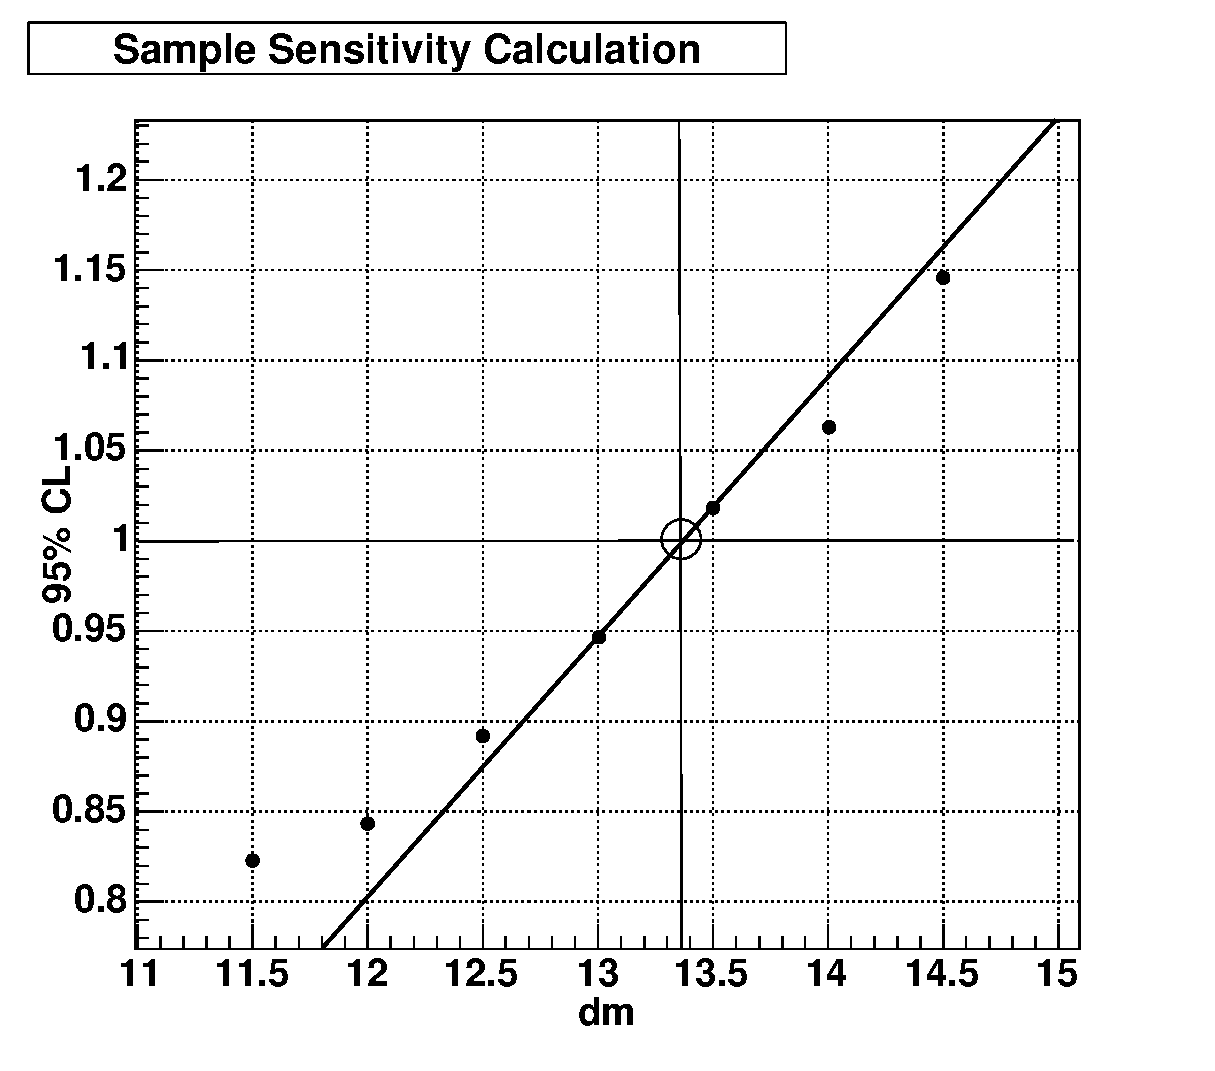
\includegraphics[width=3in]{sample.eps}
\caption{{\bf A sample sensitivity calculation.}  The sensitivity is
defined to be the value of $\Delta m$ for which the error in $D$
is 1. {\em (Dots: Step 1 and 2; Line: Step 3, Circle: Step 4.)}}
\label{sample}
\end{center}
\end{figure}

%%%%%%%%%%%%%%%%%%%%%%%%%%%%%%%%%%%%%%%%%%%%%%%%%%%%%%%%%%%%%%%%%%%%%%%%%%%%
\section{Results}

Using the Monte Carlo, fitting, and sensitivity calculation methods outlined above, we
were able to test variations to the detector parameters to
determine how they would affect error in a measurement of
dilution, regardless of the value of $\Delta m$. Sensitivity of a
dilution measurement was tested under the following conditions:
Variations in proper time resolution $\sigma_t$, variations in
dilution $D$, and variations in lifetime-dependent resolution
$\sigma_n$.
%In the first two cases, the Condor batch scheduler~\cite{condor} was used to run the series of tests on the OUHEP cluster~\cite{ouhep}, and in the last case, PBS~\cite{pbs} was used to run the series of tests at OSCER~\cite{oscer}.
Each sensitivity value represents a run of 20 generate-and-fit
iterations (4000 events each), with $\Delta m$ varied between 0
and $\sim$20 over the course of each run, as described in
Section~\ref{calcsens}.  Values used are intended to be similar to
those found at the Fermilab D\O\ detector.

\subsection{Variations in Proper Time Resolution, $\sigma_t$}

{\renewcommand{\arraystretch}{1.25}
\begin{table}
\begin{center}
\caption{{\bf Sensitivity of $D$ to variations in $\sigma_t$, 4000 events. }$\sigma_t$ was set to 0.08, 0.10, and 0.12 in the MC, and then for each of these, the fit was done with $\sigma_t$ fixed at the values listed in the Fit column.  The calculated sensitivities are given in the table.}
\label{Tts}
\vspace{0.25cm}
\begin{tabular}{|c||@{\hspace{1cm}}c@{\hspace{1cm}}|@{\hspace{1cm}}c@{\hspace{1cm}}|@{\hspace{1cm}}c@{\hspace{1cm}}|}
    \hline\hline
    $\sigma_t$ Fit $\downarrow$ $\backslash$ MC $\rightarrow$ & 0.08 & 0.10 & 0.12 \\
    \hline\hline
    0.08 & 22.07 & 23.56 & - \\
    \hline
    0.10 & 17.66 & 17.74 & 17.88 \\
    \hline
    0.12 & - & 15.74 & 15.00 \\
    \hline\hline
\end{tabular}
\end{center}
\end{table}
}

The effect of $\pm$ 20\% variations in $\sigma_t$ on the
sensitivity of $D$ are enumerated in Table \ref{Tts}.  Here, the
dilution was set to 0.16 both in the MC and as an initial value in
the fit, and time-dependent smearing was not used. $\sigma_t$ was
set to values of 0.08, 0.10, and 0.12 in the MC, and for each of these,
fitting was done with $\sigma_t$ values of 0.08, 0.10, and 0.12.  The
combinations for which the listed sensitivity is blank were not
tested.

\subsection{Variations in Dilution, $D$}

{\renewcommand{\arraystretch}{1.25}
\begin{table}
\begin{center}
\caption{{\bf Sensitivity of $D$ to variations in $D$, 4000 events. }$D$ was set to 0.128, 0.160, and 0.192 in the MC, and then for each of these, a fit was done with $D$ set to the initial values listed in the Fit column.  The calculated sensitivities are given in the table.}
\label{Td} \vspace{0.25cm}
\begin{tabular}{|c||@{\hspace{1cm}}c@{\hspace{1cm}}|@{\hspace{1cm}}c@{\hspace{1cm}}|@{\hspace{1cm}}c@{\hspace{1cm}}|}
    \hline\hline
    $D$ Fit $\downarrow$ $\backslash$ MC $\rightarrow$ & 0.128 & 0.160 & 0.192 \\
    \hline\hline
    0.128 & 16.35 & 16.35 & - \\
    \hline
    0.160 & 17.75 & 17.74 & 17.75 \\
    \hline
    0.192 & - & 18.90 & 18.91 \\
    \hline\hline
\end{tabular}
\end{center}
\end{table}
}

The effect of $\pm$ 20\% variations in the value of $D$ in the MC
vs. the initial value of $D$ used in fitting, on the sensitivity
of a measurement of $D$, are listed in Table \ref{Td}.  Here,
$\sigma_t$ was set to 0.10 both in the MC and in the fit, and
time-dependent smearing was not used. $D$ was set to values of
0.128, 0.160, and 0.192 in the MC, and for each of these, fitting was done
with $D$ at an initial values of 0.128, 0.160, and 0.192.  The
combinations for which the listed sensitivity is blank were not
tested.

\subsection{Variations in Lifetime-dependent Resolution, $\sigma_n$ \label{varsign}}

{\renewcommand{\arraystretch}{1.25}
\begin{table}
\begin{center}
\caption{{\bf Sensitivity of $D$ to variations in $\sigma_n$, 4000 events.} $\sigma_n$ was set to 0.130, 0.163, and 0.196 in the MC, and for each of these, fits were done using various methods to account for $sigma_n$ since it couldn't be included directly in the fit. These methods are listed in the Fit column, and the resulting sensitivities are given in the table.}
\label{Ttn} \vspace{0.25cm}
\begin{tabular}{|c||@{\hspace{1cm}}c@{\hspace{1cm}}|@{\hspace{1cm}}c@{\hspace{1cm}}|@{\hspace{1cm}}c@{\hspace{1cm}}|}
    \hline\hline
    $\sigma_n$ Fit $\downarrow$ $\backslash$ MC $\rightarrow$ & 0.130 & 0.163 & 0.196 \\
    \hline\hline
    $\sigma_n$ ignored & 17.799 & 17.783 & 17.808 \\
    \hline
    Avg.($\sigma_n,\sigma_t$) & 6.473 & 5.840 & 5.162 \\
    \hline
    Eff. $\sigma$ at $t$ & - & 13.386 & - \\
    \hline\hline
\end{tabular}
\end{center}
\end{table}
}

Table \ref{Ttn} lists sensitivity of a measurement of $D$ to $\pm$
20\% variations in $\sigma_n$ vs. variations in accounting for
$\sigma_n$ in fitting\footnote{$\sigma_{\mbox{\tiny eff}} = \sqrt{\sigma_t^2 +
(\sigma_n t)^2} = 0.14$ for $\sigma_t=0.10$ and $t = 0.6$, as
experimentally determined at D\O.}.  Although the MC makes it easy to
include the time-dependent smearing $\sigma_n$, this extra
Gaussian is not so easily included into the fit function.
Therefore, we chose three methods of accounting for this extra
factor in the fitting.\\

\noindent In the first row of Table \ref{Ttn}, the
time-dependent smearing is ignored altogether and
\mbox{$\sigma_{\mbox{\tiny eff}}$ = $\sigma_t$}.  In the second row, the
lifetime values from the MC were histogrammed, and then a
bin-weighted average was used to determine an average effective
value of $\sigma$ to use in the fit.  In the last row, the actual
effective smearing at each lifetime $t$ was computed during
fitting, using $\sigma_n = 0.163$. Variations were not tested.  
This is the most realistic scenario for which we have calculated sensitivity. In
all cases, $\sigma_t$ was set to 0.10 in the MC and fit, and $D$
was set to 0.160 both in the MC and for the initial fit value.

%%%%%%%%%%%%%%%%%%%%%%%%%%%%%%%%%%%%%%%%%%%%%%%%%%%%%%%%%%%%%%%%%%%%%%%%%%%%
\section{Conclusion}

The most realistic value we have determined for the sensitivity of
a measurement of dilution using an unbinned likelihood amplitude
fitting method is $\Delta m < 13.386ps^{-1}$.  This means that
with the parameters and method we have used, even in such ideal
situations as the toy MC simulates, a measurement of dilution
would not be possible for $\Delta m \geq 13.386ps^{-1}$, because
the error would be too high.  Since current experiments have set
the lower limit of $\Delta m$ above this value, at $\Delta m \geq
14.6ps^{-1}$, this measurement may not be possible using this
method.  However, using other fitting methods or combining
multiple methods, we may be able to reduce this error and still
make a measurement of dilution, and eventually, of $\Delta m$.

%%%%%%%%%%%%%%%%%%%%%%%%%%%%%%%%%%%%%%%%%%%%%%%%%%%%%%%%%%%%%%%%%%%%%%%%%%%%
%\section{}

%%%%%%%%%%%%%%%%%%%%%%%%%%%%%%%%%%%%%%%%%%%%%%%%%%%%%%%%%%%%%%%%%%%%%%%%%%%%
\begin{thebibliography}{0}

\bibitem{Bphys} K. Anikeev {\it et al.}, ``B-Physics at the Tevatron: Run II and Beyond'' (2001) hep-ph/0201071.
\bibitem{griffiths} Griffiths, David. {\it Introduction to Elementary Particles,} John Wiley \& Sons, 1987.
\bibitem{PDG} Particle Data Group. {\it Particle Physics Booklet,} 2004.
\bibitem{root} The Root Data Analysis Framework, http://root.cern.ch/.
\bibitem{cwerf} CERNLib C335: Complex Error Function, \\http://wwwasdoc.web.cern.ch/wwwasdoc/shortwrupsdir/c335/top.html.
\bibitem{roofit} The RooFit Toolkit for Data Modeling {\em (Contains a direct C++ translation of CWERF for use with Root)}, http://roofit.sourceforge.net/.
\bibitem{minuit} CERNLib (PackLib) Long Writeup D506: MINUIT Minimization Package, http://wwwasdoc.web.cern.ch/wwwasdoc/WWW/minuit/minmain/minmain.html.
%\bibitem{condor} The Condor Project, http://www.cs.wisc.edu/condor/
%\bibitem{ouhep} Information about the OUHEP cluster: http://www-hep.nhn.ou.edu/d0/grid/.
%\bibitem{pbs} Altair PBS, http://www.altair.com/software/pbspro.htm
%\bibitem{oscer} OU Supercomputing Center for Education and Research, http://www.oscer.ou.edu/.
%\bibitem{}
\end{thebibliography}

%\newpage
%%%%%%%%%%%%%%%%%%%%%%%%%%%%%%%%%%%%%%%%%%%%%%%%%%%%%%%%%%%%%%%%%%%%%%%%%%%%
%\begin{appendix}
%{\Large \bf \noindent Appendices}
%\section{Citations \label{cites}}
%
%I cited \cite{root} and all I got was this stupid citation.
%\end{appendix}
%%%%%%%%%%%%%%%%%%%%%%%%%%%%%%%%%%%%%%%%%%%%%%%%%%%%%%%%%%%%%%%%%%%%%%%%%%%%


\end{document}
